\chapter{Motivazioni alla base del lavoro}\label{ch:capitolo1}
\section{Machine Learning}
Negli ultimi decenni il Machine Learning si è imposto diventando uno dei pilastri della tecnologia e ricoprendo un ruolo piuttosto centrale, anche se nascosto, della nostra vita quotidiana. La crescita di questo settore è destinata a non fermarsi presto sopratutto grazie alla sempre maggiore quantità di dati che diventano disponibili.\\
L'idea di base è quella dell'\textit{apprendimento automatico}, ovvero fornire ai computer l'abilità di imparare alcune operazioni senza essere esplicitamente programmati, sviluppando una propria logica basata solo ed esclusivamente su dei set di dati che vengono elaborati con degli algoritmi. \\
Le varie tecniche di apprendimento si classificano in tre diversi gruppi \cite{AI}:
\begin{itemize}
	\item \textbf{Apprendimento supervisionato} i dati che vengono forniti al modello sono costituiti da una coppia di informazioni: un possibile input e il relativo output. Il sistema in questo caso deve estrarre una regola generale per associare ad ogni input il corrispettivo output corretto.
	\item \textbf{Apprendimento non supervisionato} vengono forniti al modello soltanto gli input senza i relativi output. Il sistema dovrà quindi identificare un pattern per cercare di effettuare ragionamenti e previsioni sugli input successivi. Le classi in questo caso dovranno essere apprese in maniera autonoma. 
	\item \textbf{Apprendimento per rinforzo} non ci sono dati. Il modello deve interagire con un ambiente dinamico nel quale cerca di raggiungere un obiettivo (ad esempio il superamento di un livello in un videogioco o la guida di un veicolo) ricevendo soltanto una valutazione sulle sue azioni e non informazioni su quali azioni compiere e quando compierle.
\end{itemize}
\subsection{Reti Neurali e Deep Learning}
Tra i diversi approcci e tecniche per la progettazione e l'implementazione di sistemi per l'apprendimento automatico troviamo le \textit{reti neurali} e il \textit{deep learning}.\\\\
Una \textit{rete neurale} o neural network è un sistema di apprendimento che utilizza una rete di funzioni per comprendere e tradurre un input di dati di una forma in un output desiderato, solitamente in un'altra forma. Una rete neurale è composta da elementi chiamati neuroni disposti su vari livelli, questi ricevono degli stimoli e li elaborano attivando o meno le loro uscite.  Normalmente gli strati che formano la rete sono tre (vedi figura 1.1), il primo livello detto \textit{input units} è composto dai neuroni che ricevono i segnali dall'ambiente esterno, il secondo strato,\textit{hidden units}, può essere composto anche da più colonne di neuroni e si preoccupa dell'elaborazione vera e propria, l'ultimo strato invece \textit{output units} fornisce la risposta della rete.\\
Il concetto di rete neurale artificiale ha preso ispirazione dalla biologia umana in particolare dal modo in cui funzionano e collaborano i neuroni del cervello umano per comprendere gli input sensoriali \cite{neuralnet}.\\\\ 
Il \textit{Deep Learning}, o apprendimento approfondito, è il ramo più avanzato del Machine Learning. Si tratta di un insieme di tecniche basate su reti neurali artificiali organizzate in diversi strati: ogni strato calcola i valori per quello successivo, in modo da elaborare l’informazione in maniera sempre più completa \cite{polimi}. Questo approccio trae ispirazione da alcune zone del cervello umano che si occupano della visione e dell'udito cercando di modellarne la struttura. Sopratutto per questo motivo il deep learning ha avuto maggior successo nel campo della \textit{computer vision} e del riconoscimento vocale o \textit{speech recognition}.
Se i dati a disposizione sono sufficienti il sistema è in grado di estrarre un modello corretto anche senza un pre-processamento dei dati, come invece avviene per le tecniche tradizionali di Machine Learning. In altre parole, il Deep Learning è una tecnica di apprendimento in cui reti neurali vengono esposte a vaste quantità di dati, in modo che possano imparare a svolgere compiti.\\\\
\begin{figure}
	\centering
	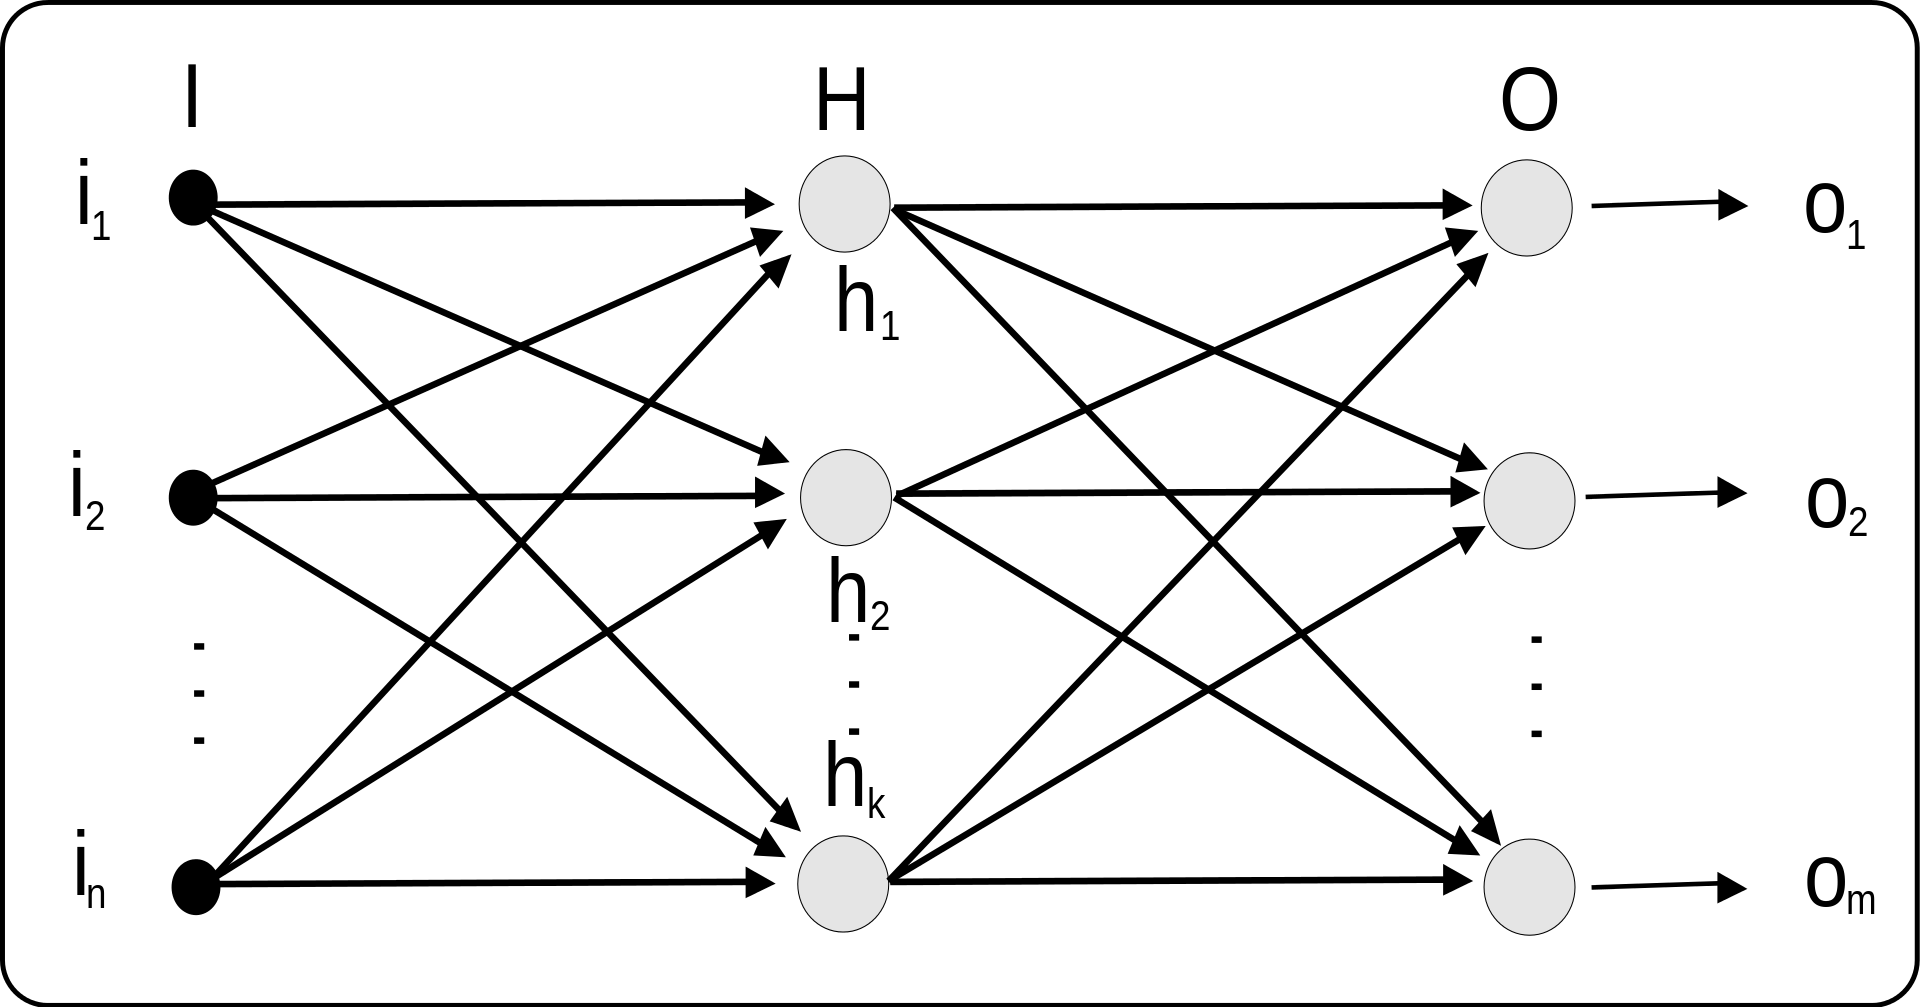
\includegraphics[width=0.8\linewidth]{../immagini/ReteNeu}
	\caption[Rete Neurale]{Struttura di una rete neurale generica }
	\label{fig:reteneu}
\end{figure}
\subsection{Il processo di apprendimento}
Come detto nel primo paragrafo, gli algoritmi di apprendimento automatico che necessitano di dati per essere applicati sono quelli supervisionati e non supervisionati. La fase di apprendimento avviene con i seguenti passaggi \cite{ML}: 
\begin{itemize}
	\item \textbf{Pre-elaborazione}: i dati, per essere forniti come input al modello, devono essere trasformati pertanto la pre-elaborazione dei dati è uno dei passi cruciali di qualsiasi applicazione di apprendimento automatico. Dai dati grezzi possiamo estrarre alcune caratteristiche significative che possono essere, nel caso in cui i dati siano delle immagini, i colori, la tonalità, l'altezza la larghezza e la profondità. Molti algoritmi di apprendimento automatico richiedono anche che, per ottenere le massime prestazioni, le caratteristiche scelte adottino la stessa scala, il che spesso viene ottenuto trasformando le caratteristiche in un intervallo [0, 1]. \\
	Per determinare	la bontà del nostro algoritmo spesso si decide di suddividere il dataset in due set distinti, uno di addestramento e uno di test. Useremo il primo per informare e ottimizzare il modello mentre teniamo da parte il secondo per valutare il modello finale.
	\item \textbf{Inizializzazione del modello}: bisogna assegnare dei valori ai parametri del modello, questi possono essere scelti randomicamente oppure ereditati da altri modelli di deep learning.  
	\item \textbf{Training}: ogni dato viene fornito in ingresso al modello il quale calcola una \textit{score function} che assegna al dato diversi punteggi (nel caso di classificatore posso essere i valori di appartenenza alle sue categorie) in seguito viene valutata anche la differenza tra valori predetti e quelli reali.
	\item \textbf{Test}: la rete processa i dati di test e viene eseguita anche una valutazione del modello. 
\end{itemize}
\begin{figure}[h!]
	\centering
	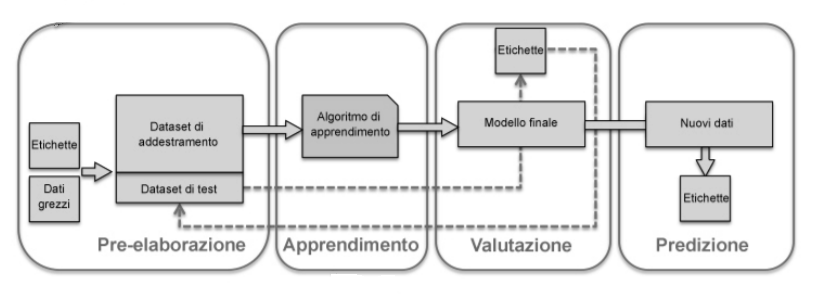
\includegraphics[width=1.1\linewidth]{../immagini/mlprocess}
	\caption[Processo di apprendimento]{Tipico diagramma di flusso per l'impiego dell'apprendimento automatico }
	\label{fig:mlprocess}
\end{figure}
La presenza di dati è quindi fondamentale per supervisionare il training e questi devono essere forniti in quantità sufficiente o altrimenti, se il campione di dati è troppo piccolo o la qualità dei dati non rappresenta correttamente la realtà, i modelli di Machine Learning saranno inutilizzabili. 
\subsection{Dataset}
Per questa ragione sono stati creati innumerevoli \textit{datasets}, sopratutto negli ultimi anni, che raccolgono enormi quantità di dati specifici per un compito con le relative annotazioni. \\
Di seguito verranno presentati i dataset utilizzati come reference durante il lavoro. 
\begin{itemize}
\item Il dataset di \textbf{Matterport3D} \cite{Matter} (Figura 1.2) fornisce dati per il training riguardo scenari indoor. I dati sono stati prelevati da 90 edifici mantenendo anche una certa varietà di ambienti. Il dataset si compone di 194,400 immagini RGB-D ovvero combinazioni di immagini RGB con le loro \textit{depth image} nelle quali ad ogni pixel viene anche associata la distanza tra piano dell'immagine e oggetto corrispondente. Vengono forniti anche i dati annotati semanticamente e per ogni scena anche una \textit{mesh} dell'ambiente. 

\item \textbf{KITTI } fornisce invece un ampio set di dati riguardanti scenari outdoor. Comprende diverse categorie tra cui 'Road', 'City', 'Residential', 'Campus' e 'Person'. Per ogni sequenza vengono forniti dati grezzi, relative annotazioni e un file di calibrazione. 

\begin{figure}
	\centering
	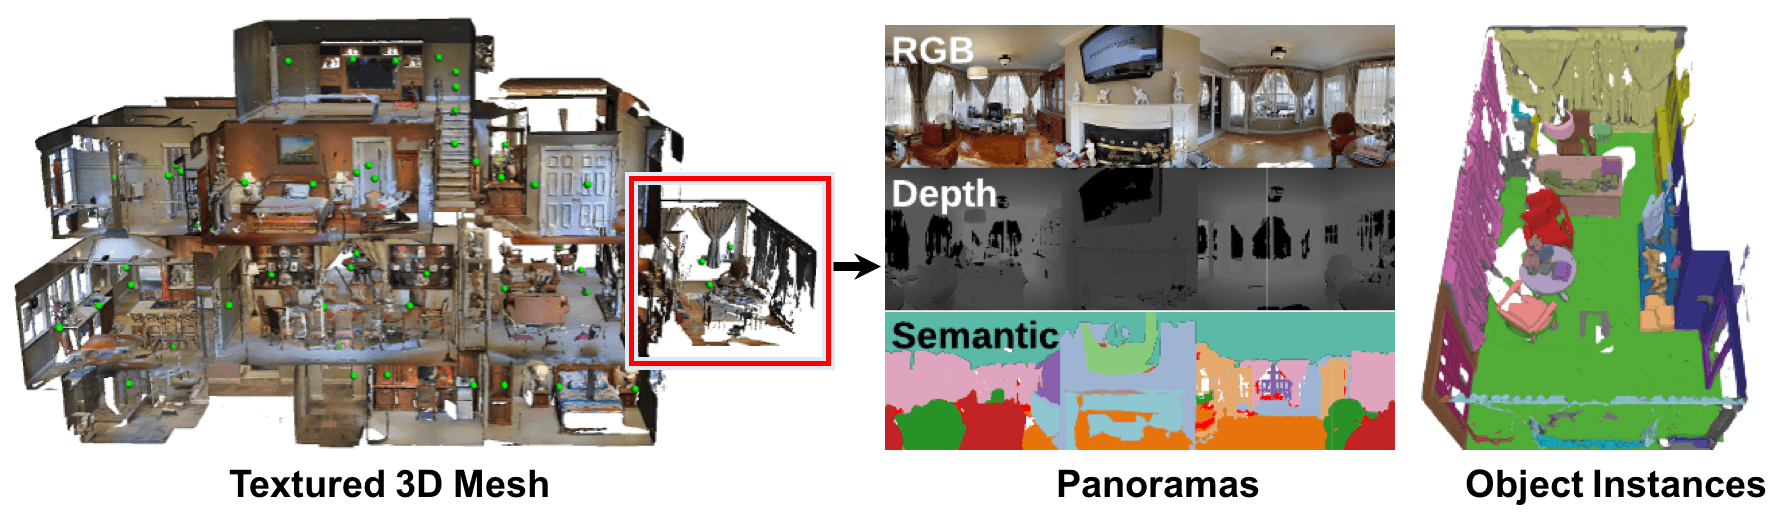
\includegraphics[width=1\linewidth]{../immagini/matterport3d}
	\caption[Matterport3d]{Il dataset Matterport }
	\label{fig:mlprocess}
\end{figure}
\end{itemize}
\section{Segmentazione semantica}
La \textit{computer vision}, anche grazie al deep learning, negli ultimi anni ha visto accrescere sempre di più l'interesse nei suoi confronti arrivando al punto in cui risulta essere molto più precisa dell'uomo in alcuni compiti \cite{Geirhos2017a}. I campi in cui questa risulta più usata sono la classificazione di immagini, il rilevamento di oggetti e la segmentazione elencati in ordine di difficoltà.\\
Se parliamo di \textit{classificazione di immagini} siamo soltanto interessati ad ottenere le etichette di tutti gli oggetti presenti in un immagine. Quando invece abbiamo a che fare con l'\textit{object detection} oltre che alla label vogliamo avere anche informazioni sulla posizione degli oggetti che ci viene fornita con dei bounding boxes ovvero dei riquadri che delimitano il soggetto. Facendo un ulteriore passo avanti in termini di precisione troviamo la \textit{segmentazione semantica} che ha come obiettivo quello di rilevare il confine esatto degli elementi nell'immagine.
\begin{figure}[h!]
	\centering
	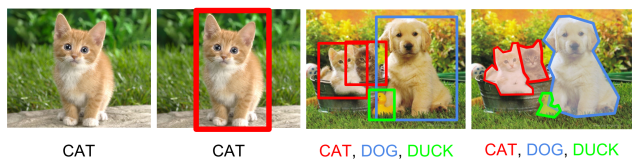
\includegraphics[width=1\linewidth]{../immagini/types}
	\caption[Task principali della Computer Vision]{Sinistra: esempio di classificazione. Immagini centrali: esempi di object detection. Destra: esempio di segmentazione semantica }
	\label{fig:types}
\end{figure}

\begin{figure}[h!]
	\centering
	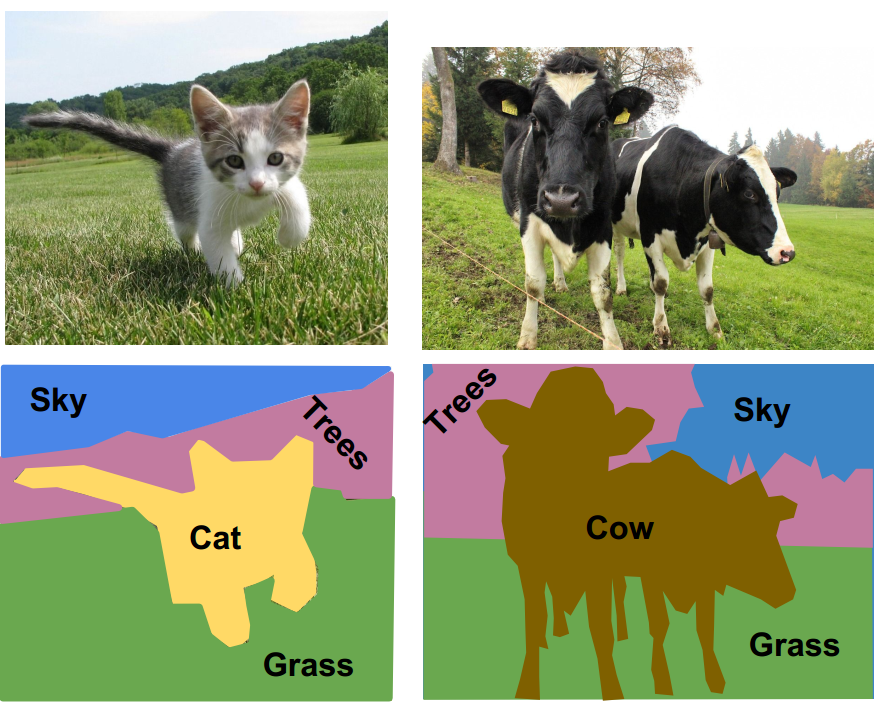
\includegraphics[width=1\linewidth]{../immagini/semantic_segmentation}
	\caption[Segmentazione semantica]{Esempio di segmentazione semantica su due immagini }
	\label{fig:types}
\end{figure}
Con la \textit{segmentazione semantica} quindi si vuole andare ad associare ad ogni pixel dell'immagine una categoria presa da un set prestabilito, nell'esempio di sinistra nella Figura 1.4 possiamo vedere che tutti i pixel appartenenti al gatto vengono colorati di giallo, tutti quelli appartenenti al terreno vengono colorati di verde, ecc. Ovviamente il numero di categorie da cui andare a pescare è arbitrario, la stessa immagine potrebbe essere segmentata anche in soltanto due categorie (una per il soggetto e una per lo sfondo). \\
La segmentazione semantica però non fa distinzione tra le varie istanze, nelle immagini di destra abbiamo due mucche, i pixel vengono assegnati indipendentemente e non c'è alcuna distinzione tra le due che però avviene se decidiamo di trattare l'immagine con un approccio di \textit{instance segmentation}.\\\\
La definizione data in precedenza vale per immagini o video, questa però può essere estesa facilmente al caso di dati 3D. In caso di \textit{point-cloud} si vuole assegnare una categoria ad ogni suo punto mentre, se i nostri dati sono sotto forma di \textit{mesh}, la categoria va assegnata ad ogni faccia.\\\\
Essendo più precisa rispetto alle altre è particolarmente indicata per quelle applicazioni nei settori che richiedono una certo livello di affidabilità come ad esempio guida autonoma, rilevazione di difetti nei materiali e prodotti, imaging medicale e nella visione robotica per identificare e muoversi tra oggetti e terreni. 
\subsection{Fase di annotazione}
La fase di annotazione è però un processo noioso, molto lento e inoltre richiede anche una certa dimestichezza con l'utilizzo di alcuni programmi. Questi problemi si aggravano nel caso in cui decidiamo di lavorare in tre dimensioni dove si aggiunge anche la difficoltà di orientarsi in uno spazio tridimensionale. Al giorno d'oggi esistono due possibili strade da percorrere quando si decide di annotare dati per un \textit{dataset} riguardante la segmentazione semantica 3D ovvero: 
\begin{itemize}
	\item \textbf{Utilizzare programmi open source} come ad esempio \textit{Blender} o \textit{MeshLab} che però richiedono una certa esperienza nell'utilizzo di motori grafici 3D. 
	\item \textbf{Affidarsi a delle aziende} che mettono a disposizione dei tool per annotare dati o che si offrono di annotarli al tuo posto, come ad esempio \textit{Scale} o \textit{Dataloop}, dietro però compenso.
\end{itemize}
Per queste ragioni è nato \textit{Shooting Labels} il primo strumento per l'annotazione semantica 3D che sfrutta la realtà virtuale per rendere più semplice e intuitiva questa fase. Utilizzando questo strumento il giocatore non necessita di nessuna competenza specifica ma indossando un headset è subito proiettato all'interno della scena nella quale utilizzando alcune armi "spara" i colori associati alle varie categorie sulle superfici etichettandole. Il lavoro diventa quindi accessibile a tutti e anche più veloce in quanto più immediata l'interazione con l'ambiente circostante rispetto all'utilizzo di altri software che non sfruttano la realtà virtuale. \\\\





